\section{Modeling the Greenland Ice Sheet Using IceBridge Data}
\subsection{Goals} %{{{
\begin{itemize}
	\item Follow an example of how to improve a coarse Greenland model by adding higher resolution Operation Icebridge (OIB) data
	\item Learn how to use the ISSM meshing tools to refine the Jakobshavn Isbr\ae (JI) basin
	\item Learn how to insert higher resolution bedrock and surface elevation data from the OIB campaign into the model within the JI basin
\end{itemize}

Go to \verb@trunk/examples/IceBridge/@ to do this tutorial.

%}}}
\subsection{Introduction}%{{{
Tutorial steps to be taken:
\begin{itemize}
	\item Refine the Greenland mesh using given JI outline.
	\item Parameterize the model, and include the high-resolution OIB bedrock and surface data.
	\item Plot the ice base and surface data.
	\item Stress Balance: run 2 inverse method runs to solve for control drag (20 steps recommended).
	\item Transient: launch 20 year runs, with coarse and refined bedrock and surface elevation data.
	\item Plot the transient results.
\end{itemize}
%}}}
\subsection{Mesh} %{{{
We modify the experiment from \href{../greenland}{the Greenland SeaRISE tutorial}, and improve from there. Run the first step in \verb@runme.m@ file to mesh the Greenland domain (similar to the previous tutorial), and plot the model. Note that the code in step 1 is interrupted after making the default mesh. Plot the model:
\begin{verbatim}>> plotmodel(md,'data','mesh');\end{verbatim}
\begin{figure}[H]
	\begin{center}
		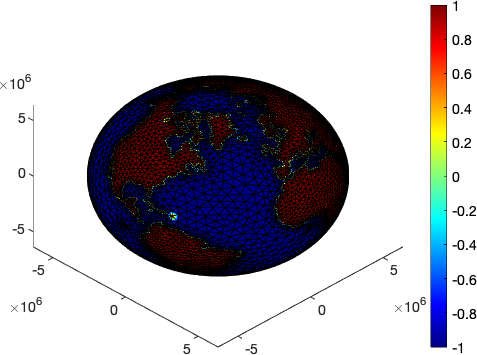
\includegraphics[scale=1.0]{../../../images/issm/documentation/tutorials/icebridge/Mesh.png}
	\end{center}
\end{figure}
Now, we want to refine the mesh in JI area. An outline of this area \verb@Jak_outline.exp@ can be found in the current directory. Use the exptool command to view this outline:
\begin{verbatim}>> exptool('Jak_outline.exp');\end{verbatim}

Next, we modify the \verb@bamg@ command by imposing a 3 km resolution within the JI area using \verb@hmaxVertices@. Note that, to implement the changes noted above you must deactivate the first occurrence of the \verb@bamg@ command in step 1, as well as the \verb@return@ command. Do this by commenting out these lines, and running step 1 again. Plot the results.
\begin{figure}[H]
	\begin{center}
		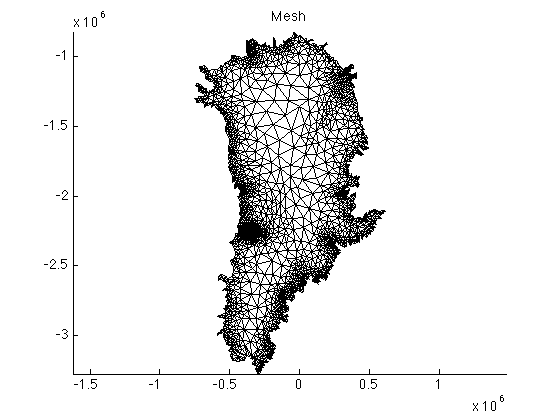
\includegraphics[scale=1.0]{../../../images/issm/documentation/tutorials/icebridge/Mesh2.png}
	\end{center}
\end{figure}
Use MATLAB's zoom tool in the figure to make a close-up of the JI domain.
%}}}
\subsection{Parameterization} %{{{
We want to include high-resolution bedrock and surface elevation data acquired in the OIB mission. The data is accessible at \href{http://data.cresis.ku.edu/data/grids/Jakobshavn_2008_2011_Composite_XYZGrid.txt}. Save the file in the \verb@../Data/@ directory.
\begin{figure}[H]
	\begin{center}
	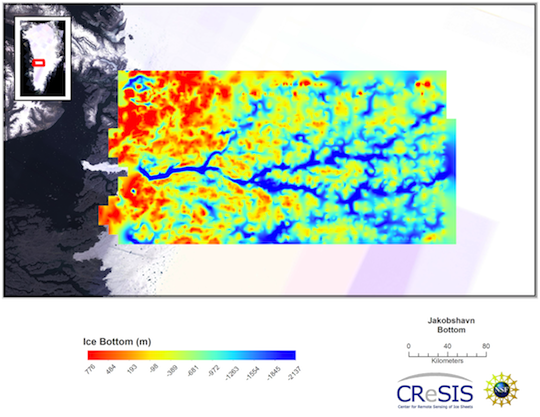
\includegraphics[scale=2.7]{../../../images/issm/documentation/tutorials/icebridge/Jakobshavn.png}
\end{center}
\end{figure}
To do this, the bedrock data is read, transformed into a usable grid, and interpolated to the mesh in the parameter file \verb@Greenland.par@:
\begin{verbatim}%Reading IceBridge data for Jakobshavn
disp('      reading IceBridge Jakobshavn bedrock');
fid  = fopen('../Data/Jakobshavn_2008_2011_Composite/grids/Jakobshavn_2008_2011_Composite_XYZGrid.txt');
titles = fgets(fid); 
data = fscanf(fid,'%g,%g,%g,%g,%g',[5 266400])';
fclose(fid);

[xi,yi]= ll2xy(md.mesh.lat,md.mesh.long,+1,45,70);
bed  = flipud(reshape(data(:,5),[360 740])); bed(find(bed==-9999))=NaN;
bedy = flipud(reshape(data(:,1),[360 740]));
bedx = flipud(reshape(data(:,2),[360 740]));

%Insert Icebridge bed and recalculate thickness
bed_jks=InterpFromGridToMesh(bedx(1,:)',bedy(:,1),bed,xi,yi,NaN);
in=ContourToMesh(md.mesh.elements,md.mesh.x,md.mesh.y,...
	   'Jak_grounded.exp','node',1);
bed_jks(~in)=NaN;
pos=find(~isnan(bed_jks));
md.geometry.base(pos)=bed_jks(pos);
md.geometry.thickness=md.geometry.surface-md.geometry.base;\end{verbatim}

Modify the \verb@Greenland.par@ file such that the surface elevation data is also included for the JI area.

\vspace{5cm}

Solution:
\begin{verbatim}%Reading IceBridge data for Jakobshavn
disp('      reading IceBridge Jakobshavn bedrock');
fid = fopen('../Data/Jakobshavn_2008_2011_Composite_XYZGrid.txt');
titles = fgets(fid); 
data = fscanf(fid,'%g,%g,%g,%g,%g',[5 266400])';
fclose(fid);

[xi,yi] = ll2xy(md.mesh.lat,md.mesh.long,+1,45,70);
bed = flipud(reshape(data(:,5),[360 740])); bed(find(bed==-9999))=NaN;
surf = flipud(reshape(data(:,4),[360 740])); surf(find(surf==-9999))=NaN;
bedy = flipud(reshape(data(:,1),[360 740]));
bedx = flipud(reshape(data(:,2),[360 740]));

%Insert Icebridge bed and recalculate thickness
bed_jks=InterpFromGridToMesh(bedx(1,:)',bedy(:,1),bed,xi,yi,NaN);
surf_jks=InterpFromGridToMesh(bedx(1,:)',bedy(:,1),surf,xi,yi,NaN);
in=ContourToMesh(md.mesh.elements,md.mesh.x,md.mesh.y,...
	   'Jak_grounded.exp','node',1);
bed_jks(~in)=NaN;
surf_jks(~in)=NaN;
pos=find(~isnan(bed_jks));
md.geometry.base(pos)=bed_jks(pos);
md.geometry.surface(pos)=surf_jks(pos);
md.geometry.thickness=md.geometry.surface-md.geometry.base;\end{verbatim}

Next, let's plot the surface elevation, the ice thickness, and base:
\begin{figure}[H]
	\begin{center}
	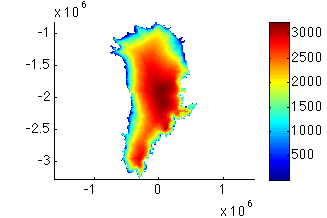
\includegraphics[scale=1.0]{../../../images/issm/documentation/tutorials/icebridge/SurfaceElevation.png}
	\caption{plotmodel(md,'data',md.geometry.surface)}
	\end{center}
\end{figure}

\begin{figure}[H]
	\begin{center}
	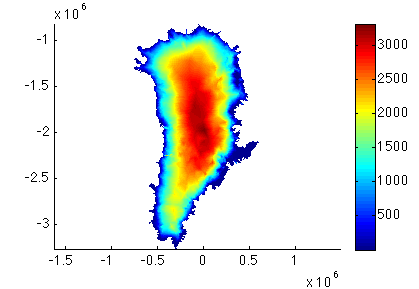
\includegraphics[scale=1.0]{../../../images/issm/documentation/tutorials/icebridge/Thickness.png}
	\caption{plotmodel(md,'data',md.geometry.thickness)}
	\end{center}
\end{figure}

\begin{figure}[H]
	\begin{center}
	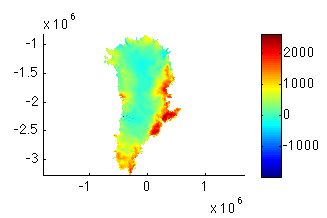
\includegraphics[scale=1.0]{../../../images/issm/documentation/tutorials/icebridge/Base.png}
	\caption{plotmodel(md,'data',md.geometry.base)}
	\end{center}
\end{figure}
To plot the difference in the ice base topography between SeaRISE and OIB datasets do (1) modify the parameterization step in your \verb@runme.m@ file by commenting out all the above lines which insert the OIB data, and change the name the model is saved under from \verb@Greenland.Parameterization2@ to \verb@Greenland.Parameterization@ and run step 2 again. A difference in the fields can be plotted using:
\begin{verbatim}>> md2=loadmodel('Models/Greenland.Parameterization2')
>> md=loadmodel('Models/Greenland.Parameterization')
>> plotmodel(md,'data',md2.geometry.base-md.geometry.base)\end{verbatim}
Zoom to the JI basin for better visibility.
\begin{figure}[H]
	\begin{center}
		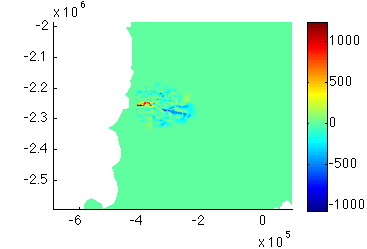
\includegraphics[scale=1.0]{../../../images/issm/documentation/tutorials/icebridge/Differences.png}
	\end{center}
\end{figure}
%}}}
\subsection{Stress Balance} %{{{
We now use inverse control methods to solve for Greenland friction coefficient. The velocity map below contains some gaps. Exclude the gaps from the inversion by creating a new \verb@*.exp@ file that outlines all the gaps in velocity data using the exptool:
\begin{verbatim}>> exptool('data_gaps.exp')\end{verbatim}

Exclude these data gaps in the inversion by giving them zero weight during the inversion process:
\begin{verbatim}in=ContourToMesh(md.mesh.elements,md.mesh.x,md.mesh.y, 'data_gaps.exp','node',1);
md.inversion.cost_functions_coefficients(find(in),1)=0.0;
md.inversion.cost_functions_coefficients(find(in),2)=0.0;\end{verbatim}

Launch the stressbalance simulation, and plot velocity and basal friction coefficient. A logarithmic
plot scale reveals more highlights of the velocity field structure:
\begin{verbatim}>> plotmodel(md,'data',md.results.StressbalanceSolution.Vel,'log',10,'caxis',[0.5 5000]);
>> plotmodel(md,'data',md.results.StressbalanceSolution.FrictionCoefficient);\end{verbatim}

They should look like this:
\begin{figure}[H]
	\begin{center}
		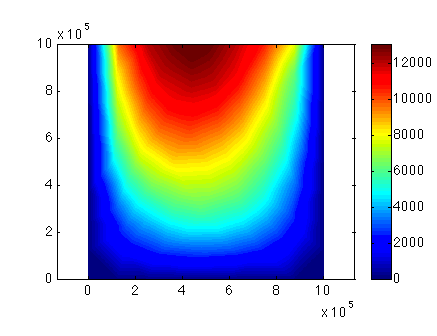
\includegraphics[scale=1.8]{../../../images/issm/documentation/tutorials/icebridge/Velocity2.png}
		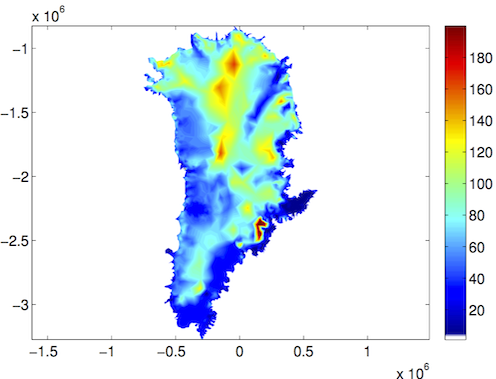
\includegraphics[scale=1.8]{../../../images/issm/documentation/tutorials/icebridge/FrictCoef.png}
	\end{center}
\end{figure}
Even at this coarse resolution we can identify the high friction values inland and lower values towards the coast, which may be related to the basal thermal regime of the ice sheet.
%}}}

\subsection{Transient} %{{{
Finally, do a transient run (step 4) for 20 years, and decrease the surface mass balance linearly by 1 m w.e./yr over the last 10 years (\verb@ncdata='../Data/Greenland_5km_dev1.2.nc';@).
\begin{verbatim}%Set surface mass balance
x1 = ncread(ncdata,'x1');
y1 = ncread(ncdata,'y1');
smb = ncread(ncdata,'smb');
smb = InterpFromGridToMesh(x1,y1,smb',md.mesh.x,md.mesh.y,0)*1000/md.materials.rho_ice;
smb = [smb smb smb-1.0];
md.smb.mass_balance = [smb;1 10 20];\end{verbatim}

Your results will be located in \verb@md.results.TransientSolution@. Plot your results using step 5. First, plot the initial plan view of velocity, surface mass balance, thickness, and surface. They should look like this:
\begin{figure}[H]
	\begin{center}
		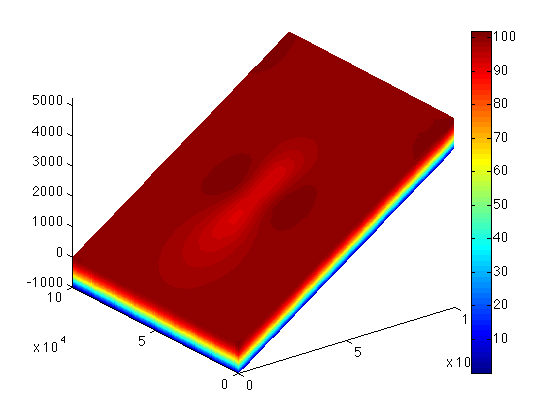
\includegraphics[scale=1.09]{../../../images/issm/documentation/tutorials/icebridge/TransientSolution.png}
	\end{center}
\end{figure}
You can plot time series of surface mass balance, mean velocity and ice volume:
\begin{figure}[H]
	\begin{center}
		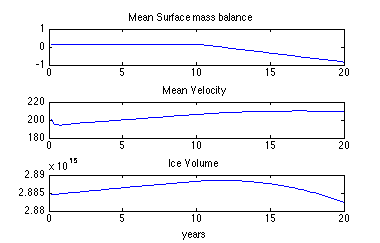
\includegraphics[scale=1.09]{../../../images/issm/documentation/tutorials/icebridge/MassVelocityVolume.png}
	\end{center}
\end{figure}

%}}}
\subsection{Results} %{{{
Well done! Here are some suggestions on what to explore further:
\begin{itemize}
	\item How would you make a plot of time series of results from the SeaRISE and IceBridge experiments?
	\item How would you make a plot of the difference between final and initial ice thickness?
\end{itemize}
%}}}
